\documentclass[]{report}

\voffset=-1.5cm
\oddsidemargin=0.0cm
\textwidth = 480pt

\usepackage{framed}
\usepackage{subfiles}
\usepackage{graphics}
\usepackage{newlfont}
\usepackage{eurosym}
\usepackage{amsmath,amsthm,amsfonts}
\usepackage{amsmath}
\usepackage{color}
\usepackage{amssymb}
\usepackage{multicol}
\usepackage[dvipsnames]{xcolor}
\usepackage{graphicx}
\begin{document}

%---------------------------------------------------------------------%

\section{Residual}
Residual (or error) represents unexplained (or residual) variation after fitting a regression model. 
It is the difference (or left over) between the observed value of the variable and the value suggested by the regression model.



\begin{itemize}
	\item The $\epsilon_i$ values 
	are called \textbf{\emph{residuals}} (they are the errors made using the
	regression model).
	\item A residual is positive when the observed value $y_i$ is greater than
	$\hat{y}_i$, the value predicted using the model.
	\item A residual is negative when the observed value $y_i$ is less than
	$\hat{y}_i$.
\end{itemize}




%%%%%%%%%%%%%%%%%%%%%%%%%%%%%%%%%%%%%%%%%%%%%%%%%%%%%%%%%%%%%%%%%%%%%%%%%


\section{Assumptions for Linear Regression}
\begin{itemize}
	\item The general assumptions underlying the regression analysis model presented in this chapter are that (1) the
	dependent variable is a random variable, and (2) the independent and dependent variables are linearly
	associated. 
	
	\item	Assumption (1) indicates that although the values of the independent variable may be controlled, the
	values of the dependent variable must be obtained through the process of random sampling.
	
	\item	If interval estimation or hypothesis testing is done in the regression analysis, three additional required assumptions are that (3) the variances of the conditional distributions of the dependent variable, given different
	values for the independent variable, are all equal, (4) the conditional distributions of the dependent variable,
	given different values for the independent variable, are all normally distributed in the population of values, and
	(5) the observed values of the dependent variable are independent of each other.
\end{itemize}


\begin{itemize}
	\item When you choose to analyse your data using linear regression, part of the process involves checking to make sure that the data you want to analyse can actually be analysed using linear regression. 
	\item You need to do this because it is only appropriate to use linear regression if your data is appropriate for six assumptions that are required for linear regression to give you a valid result.
	
	\item In practice, checking for these six assumptions just adds a little bit more time to your analysis, requiring you to click a few more buttons in \texttt{R} when performing your analysis, as well as think a little bit more about your data, but it is not a difficult task.
	
	\item Often when analysing your own data using \texttt{R}, one or more of these assumptions is violated (i.e., not met). This is not uncommon when working with real-world data rather than textbook examples, which often only show you how to carry out linear regression when everything goes well. However, even when your data fails certain assumptions, there is often a solution to overcome this. 
	\item First, let’s take a look at these six assumptions:
\end{itemize}

\begin{itemize}
	\item \textbf{Assumption 1}: Your two variables should be measured at the interval or ratio level (i.e., they are continuous). 
	
	Examples of variables that meet this criterion include revision time (measured in hours), intelligence (measured using IQ score), exam performance (measured from 0 to 100), weight (measured in kg), and so forth. 
	
	
	\item \textbf{Assumption 2}: There needs to be a linear relationship between the two variables. Whilst there are a number of ways to check whether a linear relationship exists between your two variables, we suggest creating a scatter-plot using \texttt{R}, where you can plot the dependent variable against your independent variable, and then visually inspect the scatter-plot to check for linearity. Your scatter-plot may look something like one of the following:
	
	
	
	\begin{figure}
		\centering
		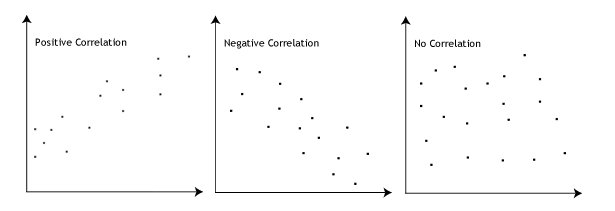
\includegraphics[width=0.7\linewidth]{images/Regre1}
		\caption{}
		\label{fig:regre1}
	\end{figure}
	If the relationship displayed in your scatterplot is not linear, you will have to either run a non-linear regression analysis or \textbf{\textit{transform}} your data, which you can do using \texttt{R}. 
	
	It is important to learn how to: \begin{itemize}
		\item[(a)] create a scatterplot to check for linearity when carrying out linear regression using \texttt{R}; \item[(b)] interpret different scatterplot results; 
		\item[(c)] transform your data using \texttt{R} if there is not a linear relationship between your two variables.
	\end{itemize} 
	
	\item \textbf{Assumption 3}: There should be no significant outliers. Outliers are simply single data points within your data that do not follow the usual pattern (e.g., in a study of 100 students’ IQ scores, where the mean score was 108 with only a small variation between students, one student had a score of 156, which is very unusual, and may even put her in the top 1\% of IQ scores globally). The following scatterplots highlight the potential impact of outliers:
	
	The problem with outliers is that they can have a negative effect on the regression equation that is used to predict the value of the dependent (outcome) variable based on the independent (predictor) variable. This will change the output that \texttt{R} produces and reduce the predictive accuracy of your results. Fortunately, when using \texttt{R} to run linear regression on your data, you can easily include criteria to help you detect possible outliers.
	\begin{figure}[h!]
		\begin{centering}
			% Requires \usepackage{graphicx}
			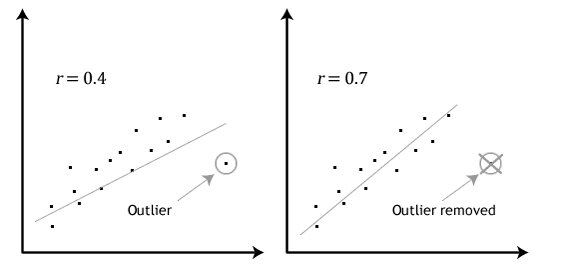
\includegraphics[width=14cm]{images/Regre2.jpg}\\
			\caption{Effect of an Outlier}
		\end{centering}
	\end{figure}
	%In our enhanced linear regression guide, we: (a) show you how to detect outliers using \textbf{case-wise diagnostics}, which is a simple process when using \texttt{R}; and (b) discuss some of the options you have in order to deal with outliers.
	
	\item \textbf{Assumption 4}: You should have independence of observations, which you can easily check using the Durbin-Watson statistic, which is a simple test to run using \texttt{R}. We explain how to interpret the result of the Durbin-Watson statistic later.
	
	\item \textbf{Assumption 5}:Your data needs to show \textbf{\textit{homoscedasticity}}, which is where the variances along the line of best fit remain similar as you move along the line. Whilst we explain more about what this means and how to assess the homoscedasticity of your data in the linear regression line, take a look at the two scatter-plots below, which provide two simple examples: one of data that meets this assumption and one that fails the assumption:
	
	\begin{figure}[h!]
		\begin{centering}
			% Requires \usepackage{graphicx}
			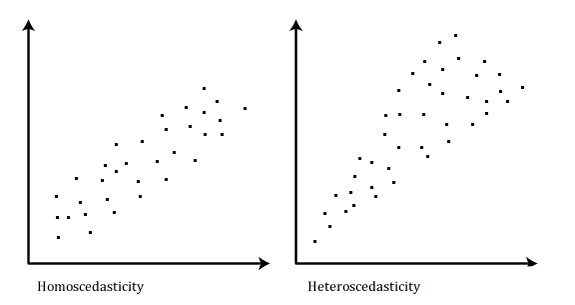
\includegraphics[width=14cm]{images/Regre3.jpg}\\
			\caption{Constant Variance}
		\end{centering}
	\end{figure}
	
	
	
	When you analyse your own data, you will be lucky if your scatterplot looks like either of the two above. Whilst these help to illustrate the differences in data that meets or violates the assumption of homoscedasticity, real-world data is often a lot more messy. 
	t b
	Therefore, in our enhanced linear regression guide, we explain: (a) some of the things you will need to consider when interpreting your data; and (b) possible ways to continue with your analysis if your data fails to meet this assumption.
	
	\item \textbf{Assumption 6}: Finally, you need to check that the residuals (errors) of your two variables are approximately normally distributed.
	
	Two common graphical methods to check this assumption include using either a histogram (with a superimposed normal curve) or by using a Normal P-P Plot. You may also use the Shapiro Wilk Test for normality.
	%  Again, in our enhanced linear regression guide, we: (a) show you how to check this assumption using \texttt{R}, whether you use a histogram (with superimposed normal curve) or Normal P-P Plot; (b) explain how to interpret these diagrams; and (c) provide a possible solution if your data fails to meet this assumption.
	
\end{itemize}

You can check assumptions all assumptions except no.1 using \texttt{R}. It is recommended to test these assumptions in this order because it represents an order where, if a violation to the assumption is not correctable, you will no longer be able to use a single linear regression (although you may be able to run another statistical test on your data instead). Just remember that if you do not run the statistical tests on these assumptions correctly, the results you get when running a linear regression might not be valid.


\begin{itemize}
	\item 
	Linear regression is the most basic and commonly used predictive analysis.  Regression estimates are used to describe data and to explain the relationship between one dependent variable and one or more independent variables.
	
	\item  At the center of the regression analysis is the task of fitting a single line through a scatter plot.  The simplest form with one dependent and one independent variable is defined by the formula y = c + b*x, where y = estimated dependent, c = constant, b = regression coefficients, and x = independent variable.
	
	\item Sometimes the dependent variable is also called a criterion variable, endogenous variable, prognostic variable, or regressand.  The independent variables are also called exogenous variables, predictor variables or regressors.
	
	\item  However linear regression analysis consists of more than just fitting a linear line through a cloud of data points.  It consists of 3 stages – (1) analyzing the correlation and directionality of the data, (2) estimating the model, i.e., fitting the line, and (3) evaluating the validity and usefulness of the model.
	
	\item 	There are 3 major uses for regression analysis – (1) causal analysis, (2) forecasting an effect, (3) trend forecasting.  Other than correlation analysis, which focuses on the strength of the relationship between two or more variables, regression analysis assumes a dependence or causal relationship between one or more independent and one dependent variable.
	
	\item 	Firstly, it might be used to identify the strength of the effect that the independent variable(s) have on a dependent variable.  Typical questions are what is the strength of relationship between dose and effect, sales and marketing spend, age and income.
	
	\item 	Secondly, it can be used to forecast effects or impacts of changes.  That is regression analysis helps us to understand how much will the dependent variable change, when we change one or more independent variables.  Typical questions are how much additional Y do I get for one additional unit X.
	
	\item Thirdly, regression analysis predicts trends and future values.  The regression analysis can be used to get point estimates.  Typical questions are what will the price for gold be in 6 month from now?  What is the total effort for a task X?
\end{itemize}





\end{document}
